\documentclass[border=6pt,tikz]{standalone}
% ===========================================================================
%  Shared drawing style for the protocol circuit figures.
%  Bold black line art on a transparent background, CM math for symbols and
%  Helvetica bold for the annotation text, matching the Keynote deck.
% ===========================================================================
\usepackage[T1]{fontenc}
\usepackage{amsmath,amssymb,braket}
\usepackage[scaled=0.94]{helvet}
\usepackage{tikz}
\usetikzlibrary{arrows.meta,decorations.pathreplacing,calc,positioning}

% ---- metrics --------------------------------------------------------------
\newcommand{\wireW}{1.0pt}      % wire line width
\newcommand{\boxW}{1.2pt}       % gate border width
\newcommand{\crossW}{3.0pt}     % swap cross width -- deliberately heavy
\newcommand{\gateR}{0.30}       % gate half-size
\newcommand{\dotR}{0.105}       % control dot radius
\newcommand{\crossR}{0.21}      % swap cross half-diagonal

% ---- annotation text ------------------------------------------------------
\newcommand{\lbl}[1]{{\sffamily\bfseries #1}}        % bold sans label
\newcommand{\lblsm}[1]{{\sffamily\bfseries\small #1}}
\newcommand{\avg}[1]{\langle #1 \rangle}
\newcommand{\note}[1]{{\sffamily\small #1}}

% ---- wire -----------------------------------------------------------------
% \qwire{y}{x_from}{x_to}
\newcommand{\qwire}[3]{\draw[line width=\wireW] (#2,#1) -- (#3,#1);}

% ---- single-qubit gate ----------------------------------------------------
% \qgate{x}{y}{label}
\newcommand{\qgate}[3]{%
  \filldraw[fill=white,line width=\boxW]
    (#1-\gateR,#2-\gateR) rectangle (#1+\gateR,#2+\gateR);
  \node at (#1,#2) {\large $#3$};}

% wider gate, for S^\dagger and similar
\newcommand{\qgatew}[3]{%
  \filldraw[fill=white,line width=\boxW]
    (#1-0.36,#2-\gateR) rectangle (#1+0.36,#2+\gateR);
  \node at (#1,#2) {$#3$};}

% ---- control dot ----------------------------------------------------------
\newcommand{\qctrl}[2]{\filldraw (#1,#2) circle (\dotR);}

% ---- vertical link between wires -----------------------------------------
% \qlink{x}{y_from}{y_to}
\newcommand{\qlink}[3]{\draw[line width=\wireW] (#1,#2) -- (#1,#3);}

% ---- SWAP target: a heavy cross ------------------------------------------
\newcommand{\qswap}[2]{%
  \draw[line width=\crossW,line cap=round]
    (#1-\crossR,#2-\crossR) -- (#1+\crossR,#2+\crossR)
    (#1-\crossR,#2+\crossR) -- (#1+\crossR,#2-\crossR);}

% ---- CNOT target ----------------------------------------------------------
\newcommand{\qtarg}[2]{%
  \filldraw[fill=white,line width=\boxW] (#1,#2) circle (0.19);
  \draw[line width=\boxW] (#1-0.19,#2) -- (#1+0.19,#2);
  \draw[line width=\boxW] (#1,#2-0.19) -- (#1,#2+0.19);}

% ---- measurement meter ----------------------------------------------------
\newcommand{\qmeter}[2]{%
  \filldraw[fill=white,line width=\boxW]
    (#1-\gateR,#2-\gateR) rectangle (#1+\gateR,#2+\gateR);
  \draw[line width=1.0pt] (#1-0.165,#2-0.095) arc (180:0:0.165);
  \draw[line width=1.0pt,-{Stealth[length=2.6mm,width=1.9mm]}]
    (#1-0.02,#2-0.135) -- (#1+0.145,#2+0.145);}

% ---- discard: a trash can -------------------------------------------------
\newcommand{\qtrash}[2]{%
  \begin{scope}[shift={(#1,#2)},line width=1.15pt,line join=round]
    \draw[rounded corners=1.2pt]
      (-0.155,0.155) -- (-0.125,-0.185) -- (0.125,-0.185) -- (0.155,0.155);
    \draw (-0.215,0.155) -- (0.215,0.155);
    \draw (-0.075,0.155) -- (-0.075,0.235) -- (0.075,0.235) -- (0.075,0.155);
    \draw[line width=0.85pt] (-0.062,0.075) -- (-0.05,-0.095);
    \draw[line width=0.85pt] (0,0.075) -- (0,-0.095);
    \draw[line width=0.85pt] (0.062,0.075) -- (0.05,-0.095);
  \end{scope}}

% ---- left brace grouping a register --------------------------------------
% \qbrace{x}{y_top}{y_bot}{label}
\newcommand{\qbrace}[4]{%
  \draw[line width=1.0pt,decorate,
        decoration={brace,amplitude=5pt,mirror,raise=0pt}]
    (#1,#2) -- (#1,#3);
  \node[left=7pt] at (#1,{(#2+#3)/2}) {\Large $#4$};}

% ---- dashed stage separator ----------------------------------------------
\newcommand{\qsep}[3]{\draw[line width=0.7pt,densely dashed,gray!65]
  (#1,#2) -- (#1,#3);}

% ---- joint measurement box spanning several wires ------------------------
% \qmeterbig{x}{y_top}{y_bot}{observable}
\newcommand{\qmeterbig}[4]{%
  \filldraw[fill=white,line width=\boxW,rounded corners=2pt]
    (#1-\gateR,#3-\gateR) rectangle (#1+\gateR,#2+\gateR);
  \draw[line width=1.0pt] (#1-0.165,{(#2+#3)/2-0.095}) arc (180:0:0.165);
  \draw[line width=1.0pt,-{Stealth[length=2.6mm,width=1.9mm]}]
    (#1-0.02,{(#2+#3)/2-0.135}) -- (#1+0.145,{(#2+#3)/2+0.145});
  \node at (#1,{(#2+#3)/2+0.46}) {$#4$};}

% ---- meter with the measured observable named beside it ------------------
% \qmeterlab{x}{y}{observable}
\newcommand{\qmeterlab}[3]{\qmeter{#1}{#2}}

% ---- gate present only in one measurement setting ------------------------
\newcommand{\qgatedash}[3]{%
  \filldraw[fill=white,draw=none]
    (#1-0.36,#2-\gateR) rectangle (#1+0.36,#2+\gateR);
  \draw[line width=\boxW,densely dashed]
    (#1-0.36,#2-\gateR) rectangle (#1+0.36,#2+\gateR);
  \node at (#1,#2) {$#3$};}

% ---- observable name set above a meter (used by the compact variants) ----
\newcommand{\qmeterover}[3]{\qmeter{#1}{#2}%
  \node[above=2pt] at (#1,#2+\gateR) {\small $#3$};}
\newcommand{\qmeterbigover}[4]{\qmeterbig{#1}{#2}{#3}{}%
  \node[above=2pt] at (#1,#2+\gateR) {\small $#4$};}

\begin{document}
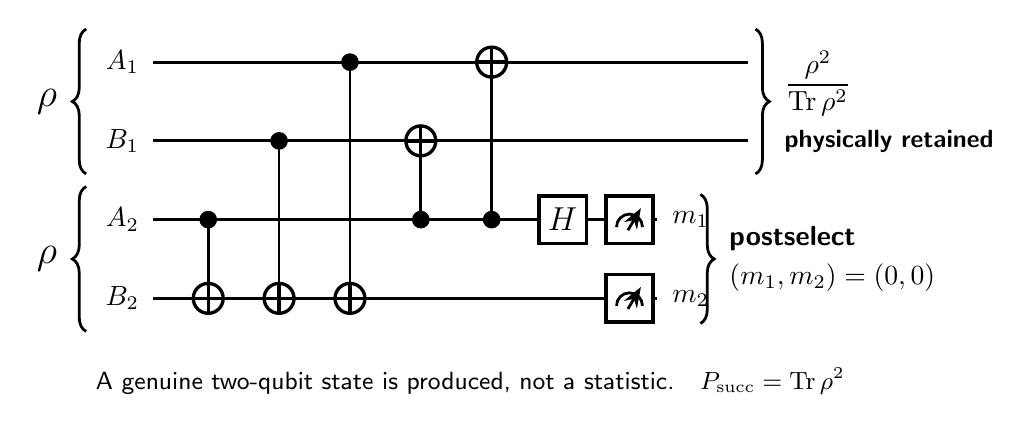
\begin{tikzpicture}[x=1cm,y=1cm]

% ---- wire rows -----------------------------------------------------------
\def\ya{3.0}   % A1  retained
\def\yb{2.0}   % B1  retained
\def\yc{1.0}   % A2  measured
\def\yd{0.0}   % B2  measured

\def\xl{1.05}  % wire start
\def\xr{8.60}  % wire end (retained pair)
\def\xm{7.45}  % wire end (measured pair)

\qwire{\ya}{\xl}{\xr}
\qwire{\yb}{\xl}{\xr}
\qwire{\yc}{\xl}{\xm}
\qwire{\yd}{\xl}{\xm}

% ---- input registers -----------------------------------------------------
\qbrace{0.20}{\ya+0.42}{\yb-0.42}{\rho}
\qbrace{0.20}{\yc+0.42}{\yd-0.42}{\rho}
\node at (0.66,\ya) {$A_1$};
\node at (0.66,\yb) {$B_1$};
\node at (0.66,\yc) {$A_2$};
\node at (0.66,\yd) {$B_2$};

% ---- the five CNOTs ------------------------------------------------------
\qlink{1.75}{\yc}{\yd}\qctrl{1.75}{\yc}\qtarg{1.75}{\yd}   % A2 -> B2
\qlink{2.65}{\yb}{\yd}\qctrl{2.65}{\yb}\qtarg{2.65}{\yd}   % B1 -> B2
\qlink{3.55}{\ya}{\yd}\qctrl{3.55}{\ya}\qtarg{3.55}{\yd}   % A1 -> B2
\qlink{4.45}{\yc}{\yb}\qctrl{4.45}{\yc}\qtarg{4.45}{\yb}   % A2 -> B1
\qlink{5.35}{\yc}{\ya}\qctrl{5.35}{\yc}\qtarg{5.35}{\ya}   % A2 -> A1

% ---- Hadamard on A2 ------------------------------------------------------
\qgate{6.25}{\yc}{H}

% ---- measurements on the lower pair --------------------------------------
\qmeter{7.10}{\yc}
\qmeter{7.10}{\yd}
\node[right=2pt] at (\xm,\yc) {$m_1$};
\node[right=2pt] at (\xm,\yd) {$m_2$};

\draw[line width=1.0pt,decorate,decoration={brace,amplitude=5pt}]
  (8.00,\yc+0.32) -- (8.00,\yd-0.32);
\node[right=7pt,align=left] at (8.00,{(\yc+\yd)/2})
  {\lbl{postselect}\\[2pt]$(m_1,m_2)=(0,0)$};

% ---- retained output -----------------------------------------------------
\draw[line width=1.0pt,decorate,decoration={brace,amplitude=5pt}]
  (\xr+0.10,\ya+0.42) -- (\xr+0.10,\yb-0.42);
\node[right=7pt,align=left] at (\xr+0.10,{(\ya+\yb)/2})
  {$\dfrac{\rho^{2}}{\operatorname{Tr}\rho^{2}}$\\[4pt]
   \lblsm{physically retained}};

% ---- footnote ------------------------------------------------------------
\node[anchor=west,align=left] at (0.20,-1.05)
  {\note{A genuine two-qubit state is produced, not a statistic.\quad
         $P_{\mathrm{succ}}=\operatorname{Tr}\rho^{2}$}};

\end{tikzpicture}
\end{document}
